% Slide 04: Identifying the Challenge
\begin{frame}{Identifying the Challenge}
    \begin{columns}[T]
        \begin{column}{0.48\textwidth}
            \begin{block}{The Problem}
                \begin{itemize}
                    \item \textbf{Challenge 1:} Lorem ipsum dolor sit amet, consectetur adipiscing elit
                    \item \textbf{Challenge 2:} Sed do eiusmod tempor incididunt ut labore
                    \item \textbf{Challenge 3:} Ut enim ad minim veniam, quis nostrud exercitation
                \end{itemize}
            \end{block}

            \vspace{0.3cm}

            \centering
            
\begin{tikzpicture}
                \draw[red,thick] (0,0) -- (2,2);
                \draw[red,thick] (2,0) -- (0,2);
                \node[below] at (1,-0.3) {\textcolor{red}{\textbf{Pain Points}}};
            \end{tikzpicture}
        \end{column}

        \begin{column}{0.48\textwidth}
            \begin{block}{Our Solution}
                \begin{itemize}
                    \item \textbf{Solution 1:} Innovative approach to address challenge 1
                    \item \textbf{Solution 2:} Proven methodology for challenge 2
                    \item \textbf{Solution 3:} Scalable platform for challenge 3
                \end{itemize}
            \end{block}

            \vspace{0.3cm}

            \centering
            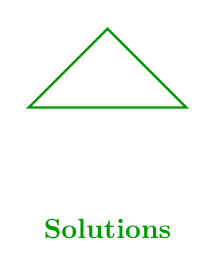
\begin{tikzpicture}
                \draw[green!60!black,thick] (0,1) -- (1,2) -- (2,1) -- cycle;
                \node[below] at (1,-0.3) {\textcolor{green!60!black}{\textbf{Solutions}}};
            \end{tikzpicture}
        \end{column}
    \end{columns}

    \vspace{0.5cm}

    \centering
    \highlight{Our solution addresses a \money{10B+} market opportunity}
\end{frame}
